% !TeX root = main.tex
% !TeX spellcheck = en_US

\documentclass[aspectratio=169,9pt]{beamer}

\usepackage{royslides}
\usepackage{graphicx}
\graphicspath{{figures/}} % Setting the graphicspath
\usepackage{subfig}
\usepackage[]{hyperref}
\usepackage{listings}

\title{ML pipelines in HEP}
\date{Milan University, 2022}
\author{Roy Stegeman}
\institute{University of Milan and INFN Milan}

% LISTINGS ====================================================================
\definecolor{mygreen}{rgb}{0,0.6,0}
\definecolor{mygray}{rgb}{0.5,0.5,0.5}
\definecolor{mymauve}{rgb}{0.58,0,0.82}

\makeatletter
\lst@CCPutMacro
    \lst@ProcessOther {"2D}{\lst@ttfamily{-{}}{-}}
    \@empty\z@\@empty
\makeatother

\lstset{ 
  backgroundcolor=\color{white},   % choose the background color; you must add \usepackage{color} or \usepackage{xcolor}; should come as last argument
  basicstyle=\footnotesize,        % the size of the fonts that are used for the code
  breakatwhitespace=false,         % sets if automatic breaks should only happen at whitespace
  breaklines=true,                 % sets automatic line breaking
  captionpos=b,                    % sets the caption-position to bottom
  commentstyle=\color{mygreen},    % comment style
  deletekeywords={...},            % if you want to delete keywords from the given language
  escapeinside={\%*}{*)},          % if you want to add LaTeX within your code
  extendedchars=true,              % lets you use non-ASCII characters; for 8-bits encodings only, does not work with UTF-8
  % firstnumber=1000,                % start line enumeration with line 1000
  frame=single,	                   % adds a frame around the code
  keepspaces=true,                 % keeps spaces in text, useful for keeping indentation of code (possibly needs columns=flexible)
  keywordstyle=\color{blue},       % keyword style
  language=Octave,                 % the language of the code
  morekeywords={*,...},            % if you want to add more keywords to the set
  numbers=left,                    % where to put the line-numbers; possible values are (none, left, right)
  numbersep=5pt,                   % how far the line-numbers are from the code
  numberstyle=\tiny\color{mygray}, % the style that is used for the line-numbers
  rulecolor=\color{black},         % if not set, the frame-color may be changed on line-breaks within not-black text (e.g. comments (green here))
  showspaces=false,                % show spaces everywhere adding particular underscores; it overrides 'showstringspaces'
  showstringspaces=false,          % underline spaces within strings only
  showtabs=false,                  % show tabs within strings adding particular underscores
  stepnumber=2,                    % the step between two line-numbers. If it's 1, each line will be numbered
  stringstyle=\color{mymauve},     % string literal style
  tabsize=2,	                   % sets default tabsize to 2 spaces
  title=\lstname                   % show the filename of files included with \lstinputlisting; also try caption instead of title
}
% ====================================================================


\begin{document}
% TITLEPAGE ====================================================================
{
\setbeamertemplate{headline}{} % remove headline from titlepage
\begin{frame}
  \titlepage
\end{frame}
}


% INTRO ========================================================================
\section{Status of ML pipelines in HEP}
\begin{frame}[t]{Experimental data pipeline}
  % \begin{itemize}
  %   \item Large dataset
  %   \item convert to training data
  %   \item training framework
  %   \item trained model
  %   \item store in database dependent format
  %   \item do inference to get results
  % \end{itemize}
  \centering
  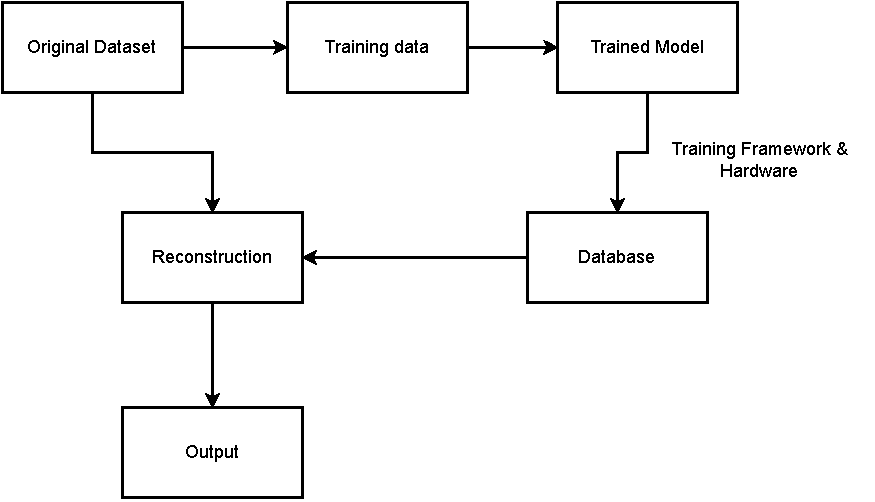
\includegraphics[width=.7\textwidth]{MLworkflow.drawio.pdf}
\end{frame}


\begin{frame}[t]{Preparing training data}
  Data preparation relies on complicated pipelines (example is simplified)
  \vspace*{1em}
  Recent developments:
  \begin{itemize}
    \item Uproot (python) gaining popularity
    \item More non-ROOT formats are used
    % \item In reality input data is Event Data Model thus more steps
  \end{itemize}
  % \begin{itemize}
  %   \item input primary data
  %   \item Convert to ROOT or HDF5/zarr
  %   \item root to uproot to numpy
  %   \item HDF5 to numpy
  % \end{itemize}
  \vspace*{-2em}
  \begin{figure}
    \centering
    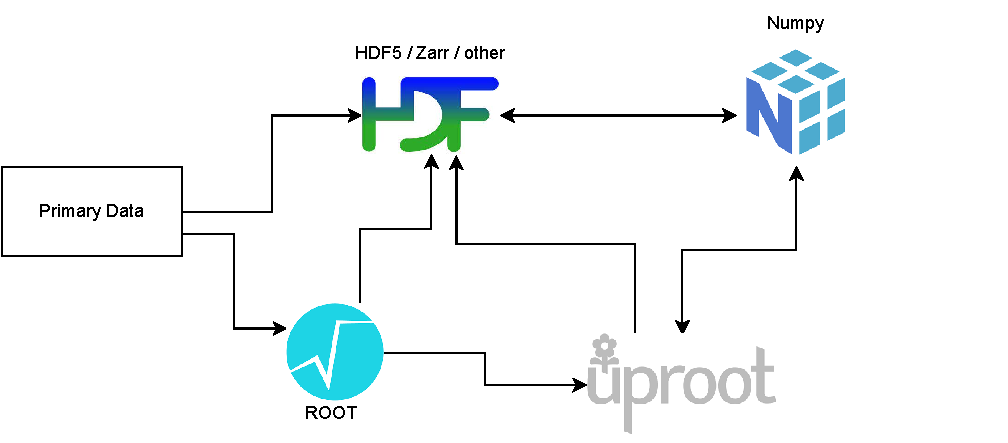
\includegraphics[width=.7\textwidth]{making_dataset.drawio.pdf}
  \end{figure}
\end{frame}


\begin{frame}[t]{Can this be simplified?}
  \begin{itemize}
    \item Different parties have different interests
    \item Experiments: lots of data available in ROOT, but\ldots
    \begin{itemize}
      \item primary data needs to be converted for training
      \item there is no consistent ROOT data format
    \end{itemize}
    \item ROOT: introduce yet another data format \href{https://root.cern/doc/master/md_tree_ntuple_v7_doc_README.html}{\color{blue}RNtuple}
    \begin{itemize}
      \item Widespread use will require standardization
    \end{itemize}
    \item Similarly no consistent HEPData format
    \item Doesn't the ML community already have a solution for this? Maybe \href{https://github.com/apache/parquet-format}{\color{blue}Parquet}
  \end{itemize}
  \vspace*{1em}
  Much to improve on the data side!\\\vspace*{1cm}
  But even if we will ever have a standardized data format, it's not all smooth sailing...
\end{frame}


\begin{frame}[t]{ML model pipeline}
  % \begin{itemize}
  %   \item Use of graph based neural networks widely spread in HEP community (particle tracking, jet tagging, clustering\ldots, pdf fits\ldots)
  %   \item Tensorflow, Keras, Scikit-learn, Pytorch, \ldots
  %   \item Conda, venv, docker, \ldots
  %   \item grid stored in tool with non-standard format
  %   \item C++ framework at (LHC) experiments
  %   \item Run models on different OS or hardware
  % \end{itemize}
  Use of graph based neural networks widely spread in HEP community \\
  (particle tracking, jet tagging, clustering\ldots, pdf fits\ldots)\\\vspace*{0.5cm}
  \begin{figure}
    \centering
    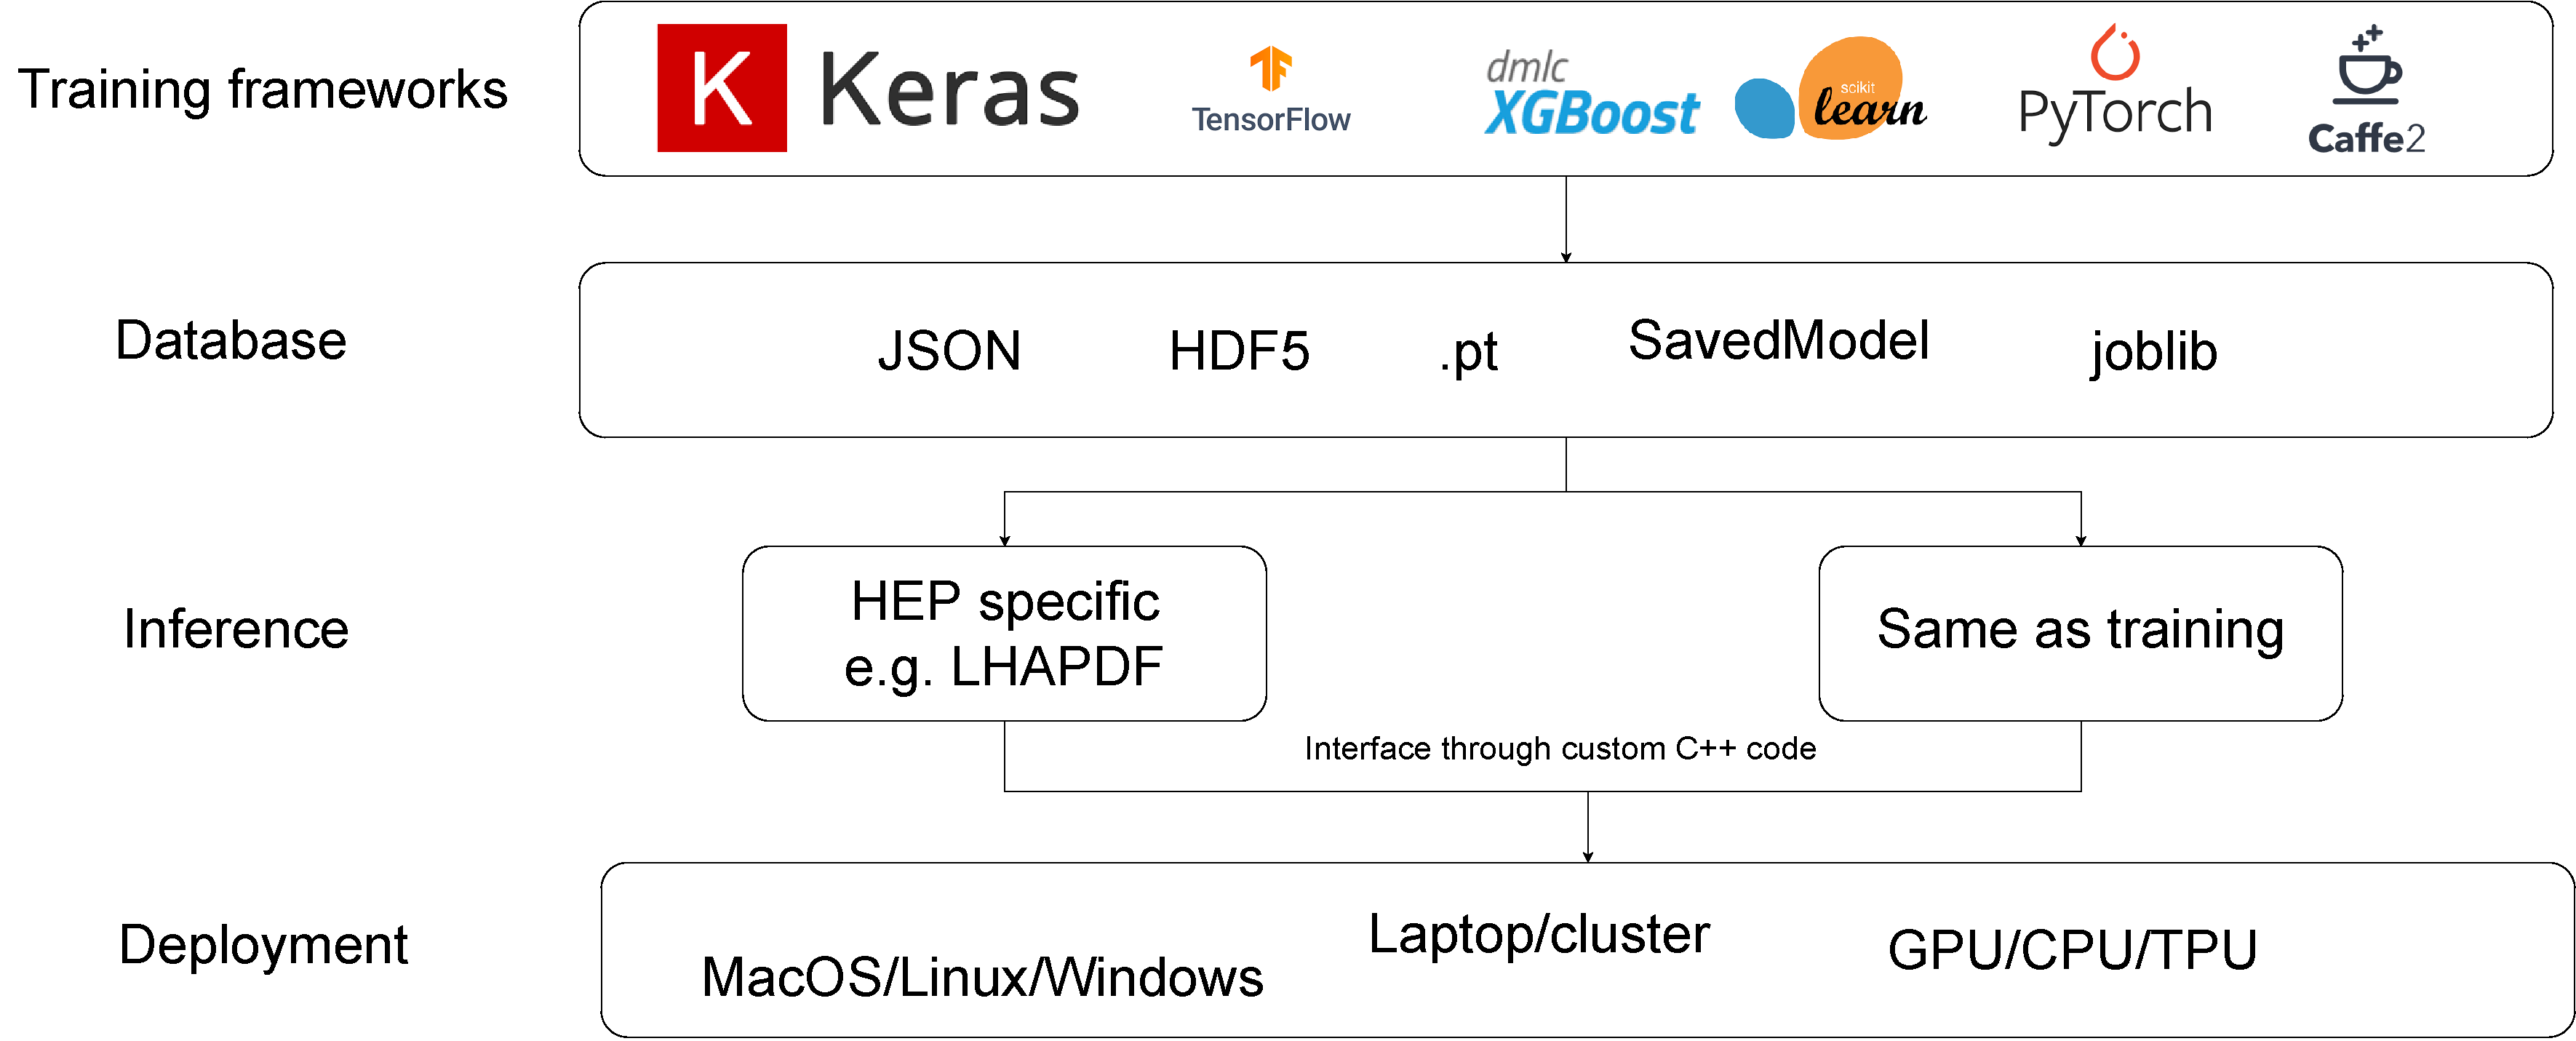
\includegraphics[width=.6\textwidth]{ml_models.pdf}
  \end{figure}
  \begin{itemize}
    \item Lack of interoperatibilty (e.g. Pytorch cannot run interference on TF trained model)
    \item Lack of consistent runtime layer for combinations of hardware and software \\ (e.g. export TF to \href{https://developer.nvidia.com/tensorrt?utm_source=thenewstack&utm_medium=website&utm_campaign=platform}{\color{blue}TensorRT} model for NVIDIA GPUs)
  \end{itemize}
\end{frame}


\begin{frame}[t]{ML model pipeline}
  % \begin{itemize}
  %   \item Use of graph based neural networks widely spread in HEP community (particle tracking, jet tagging, clustering\ldots, pdf fits\ldots)
  %   \item Tensorflow, Keras, Scikit-learn, Pytorch, \ldots
  %   \item Conda, venv, docker, \ldots
  %   \item grid stored in tool with non-standard format
  %   \item C++ framework at (LHC) experiments
  %   \item Run models on different OS or hardware
  % \end{itemize}
  Use of graph based neural networks widely spread in HEP community \\
  (particle tracking, jet tagging, clustering\ldots, pdf fits\ldots)\\\vspace*{0.5cm}
  \begin{figure}
    \centering
    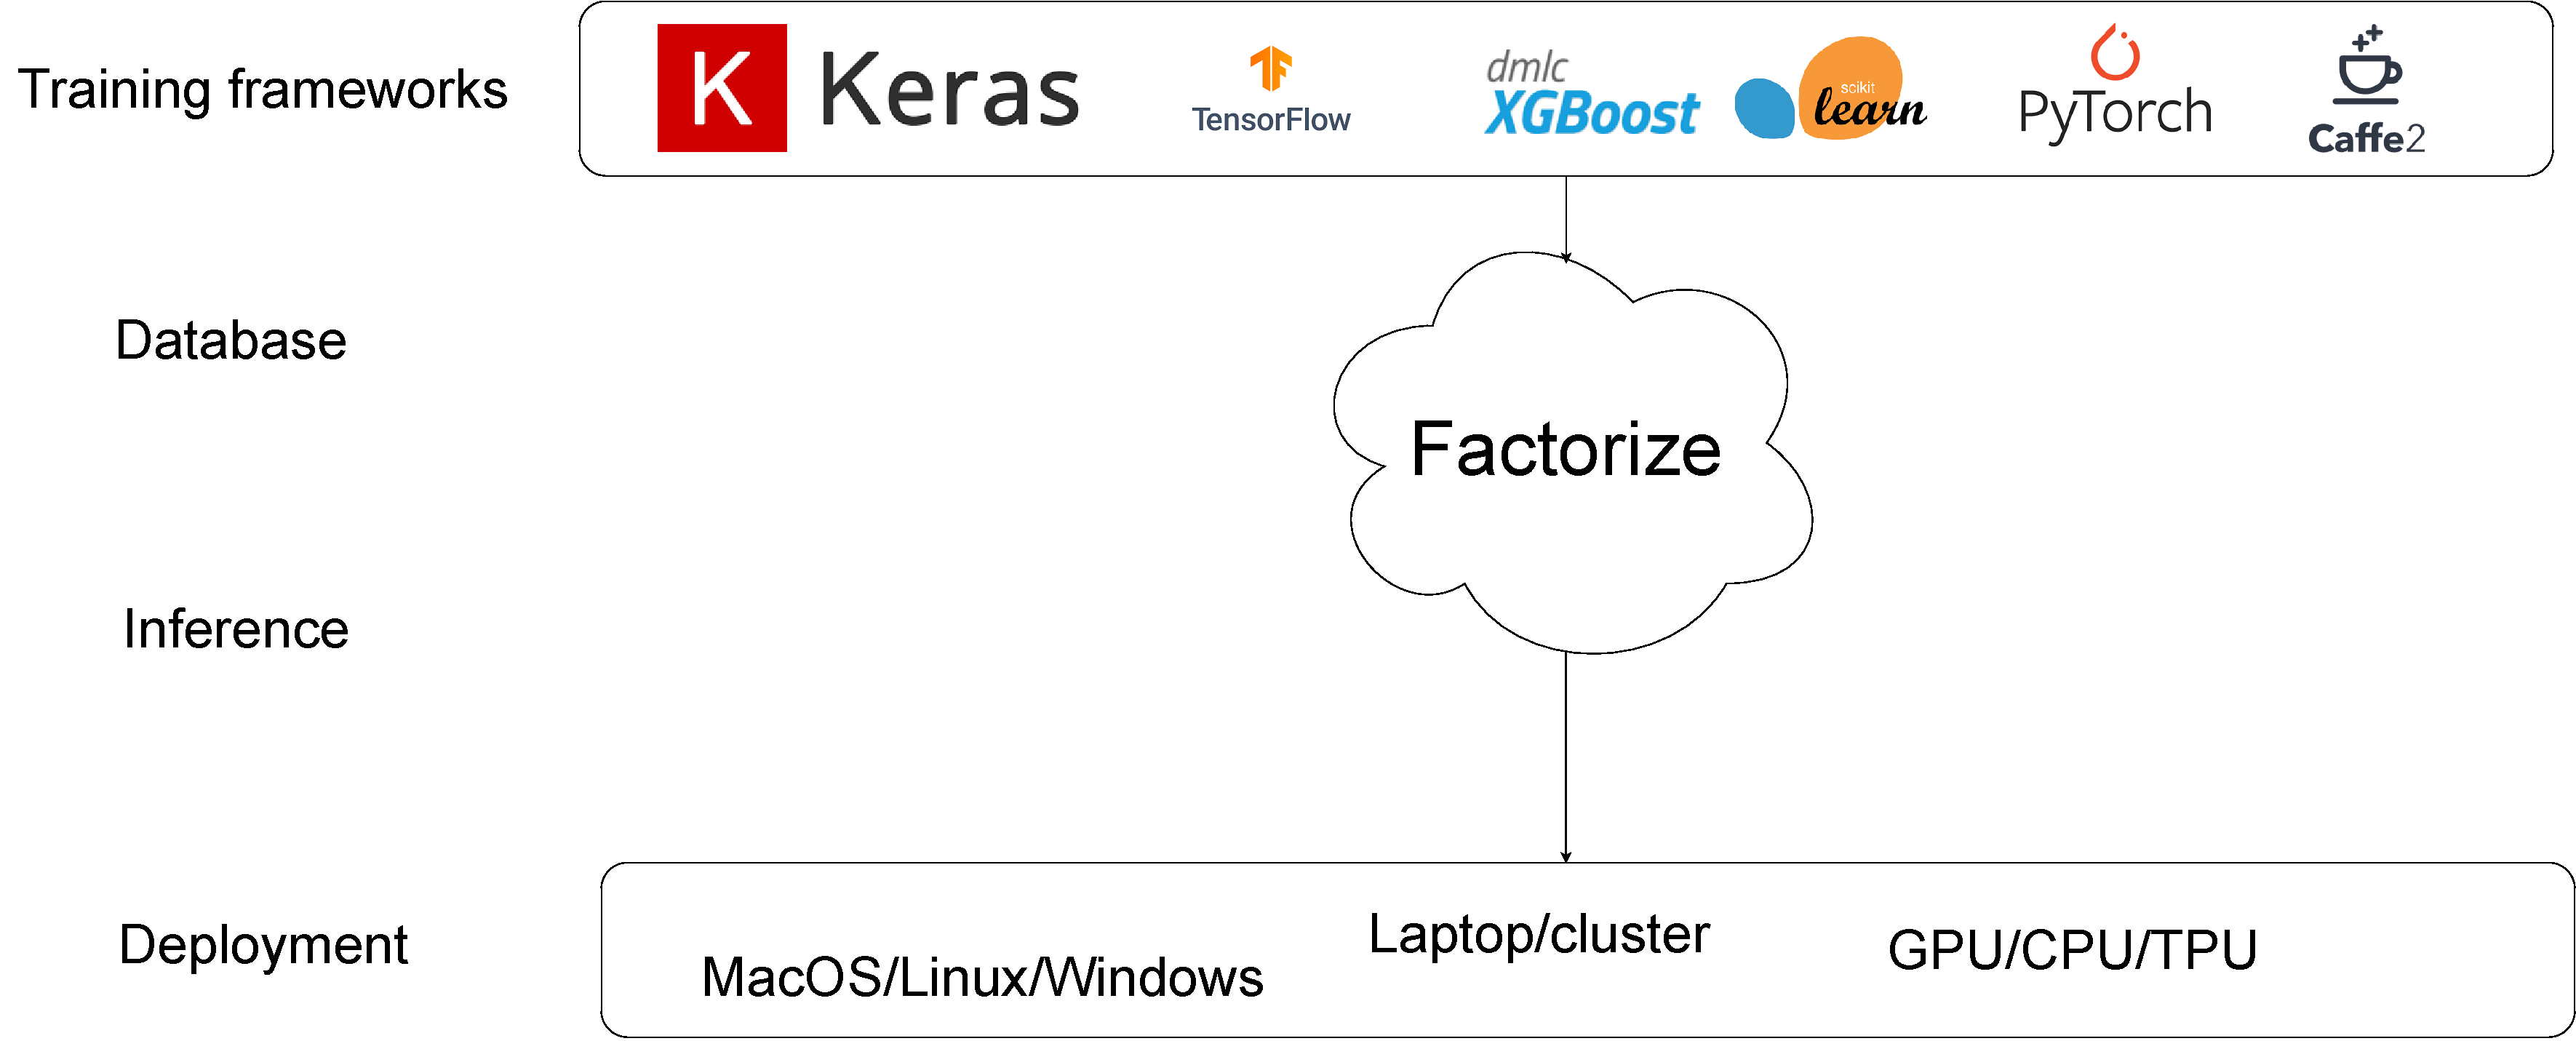
\includegraphics[width=.6\textwidth]{factorize_this_workflow.pdf}
  \end{figure}
  \begin{itemize}
    \item Only requires knowledge/installation of a single framework
    \item Tools only need to provide support for a single format
    \item Physicists waste less time writing interfaces
  \end{itemize}
\end{frame}


% ONNX =========================================================================
\section{Introducing ONNX}
\begin{frame}[t]{Machine learning pipeline}
  \begin{figure}
    \centering
    \only<1>{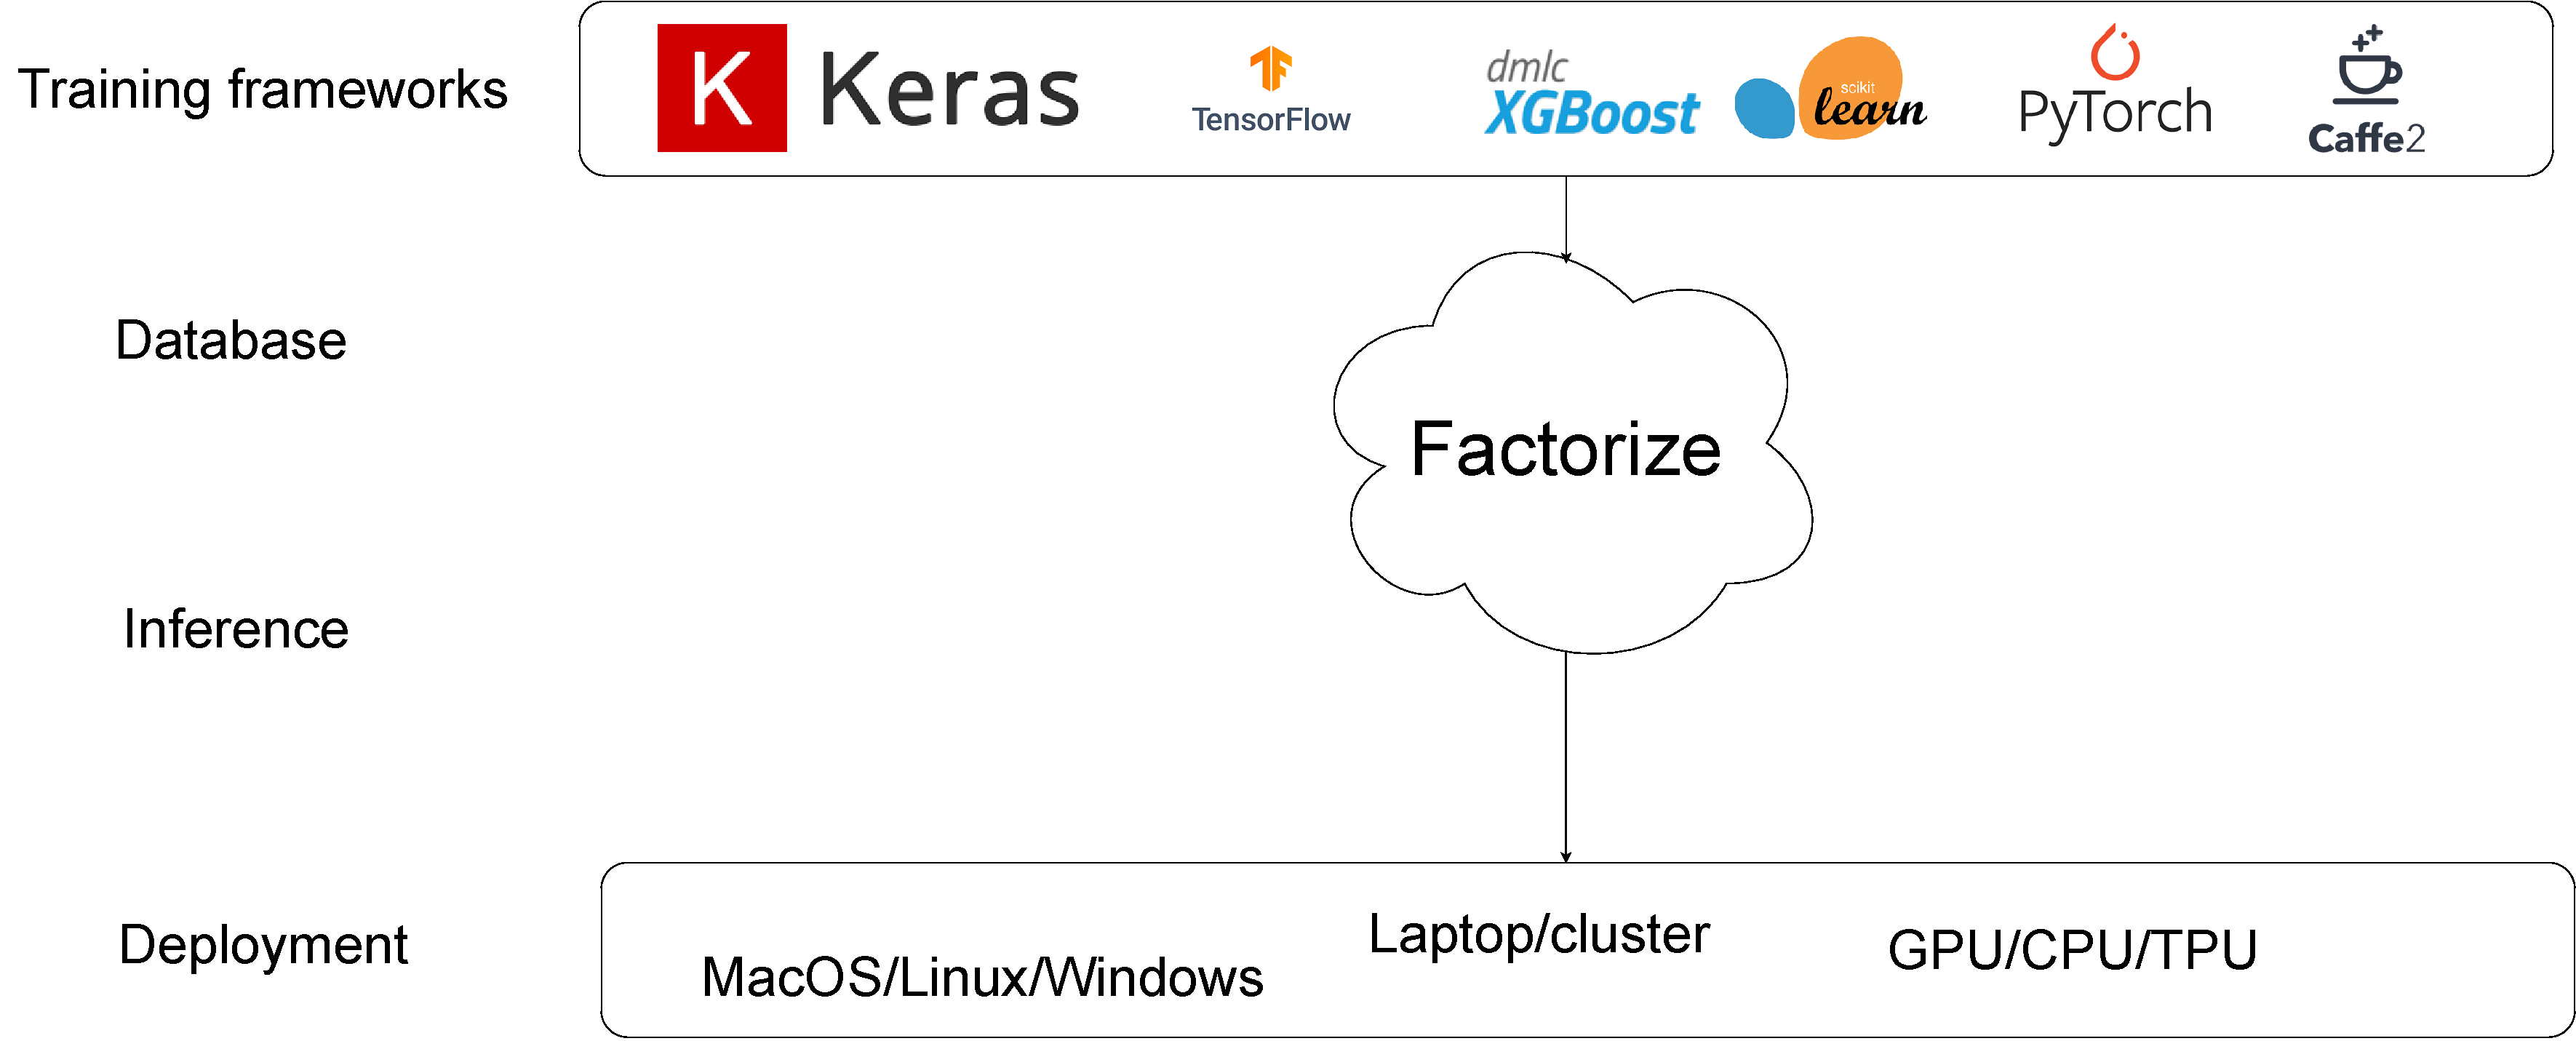
\includegraphics[width=.7\textwidth]{factorize_this_workflow.pdf}}
    \only<2>{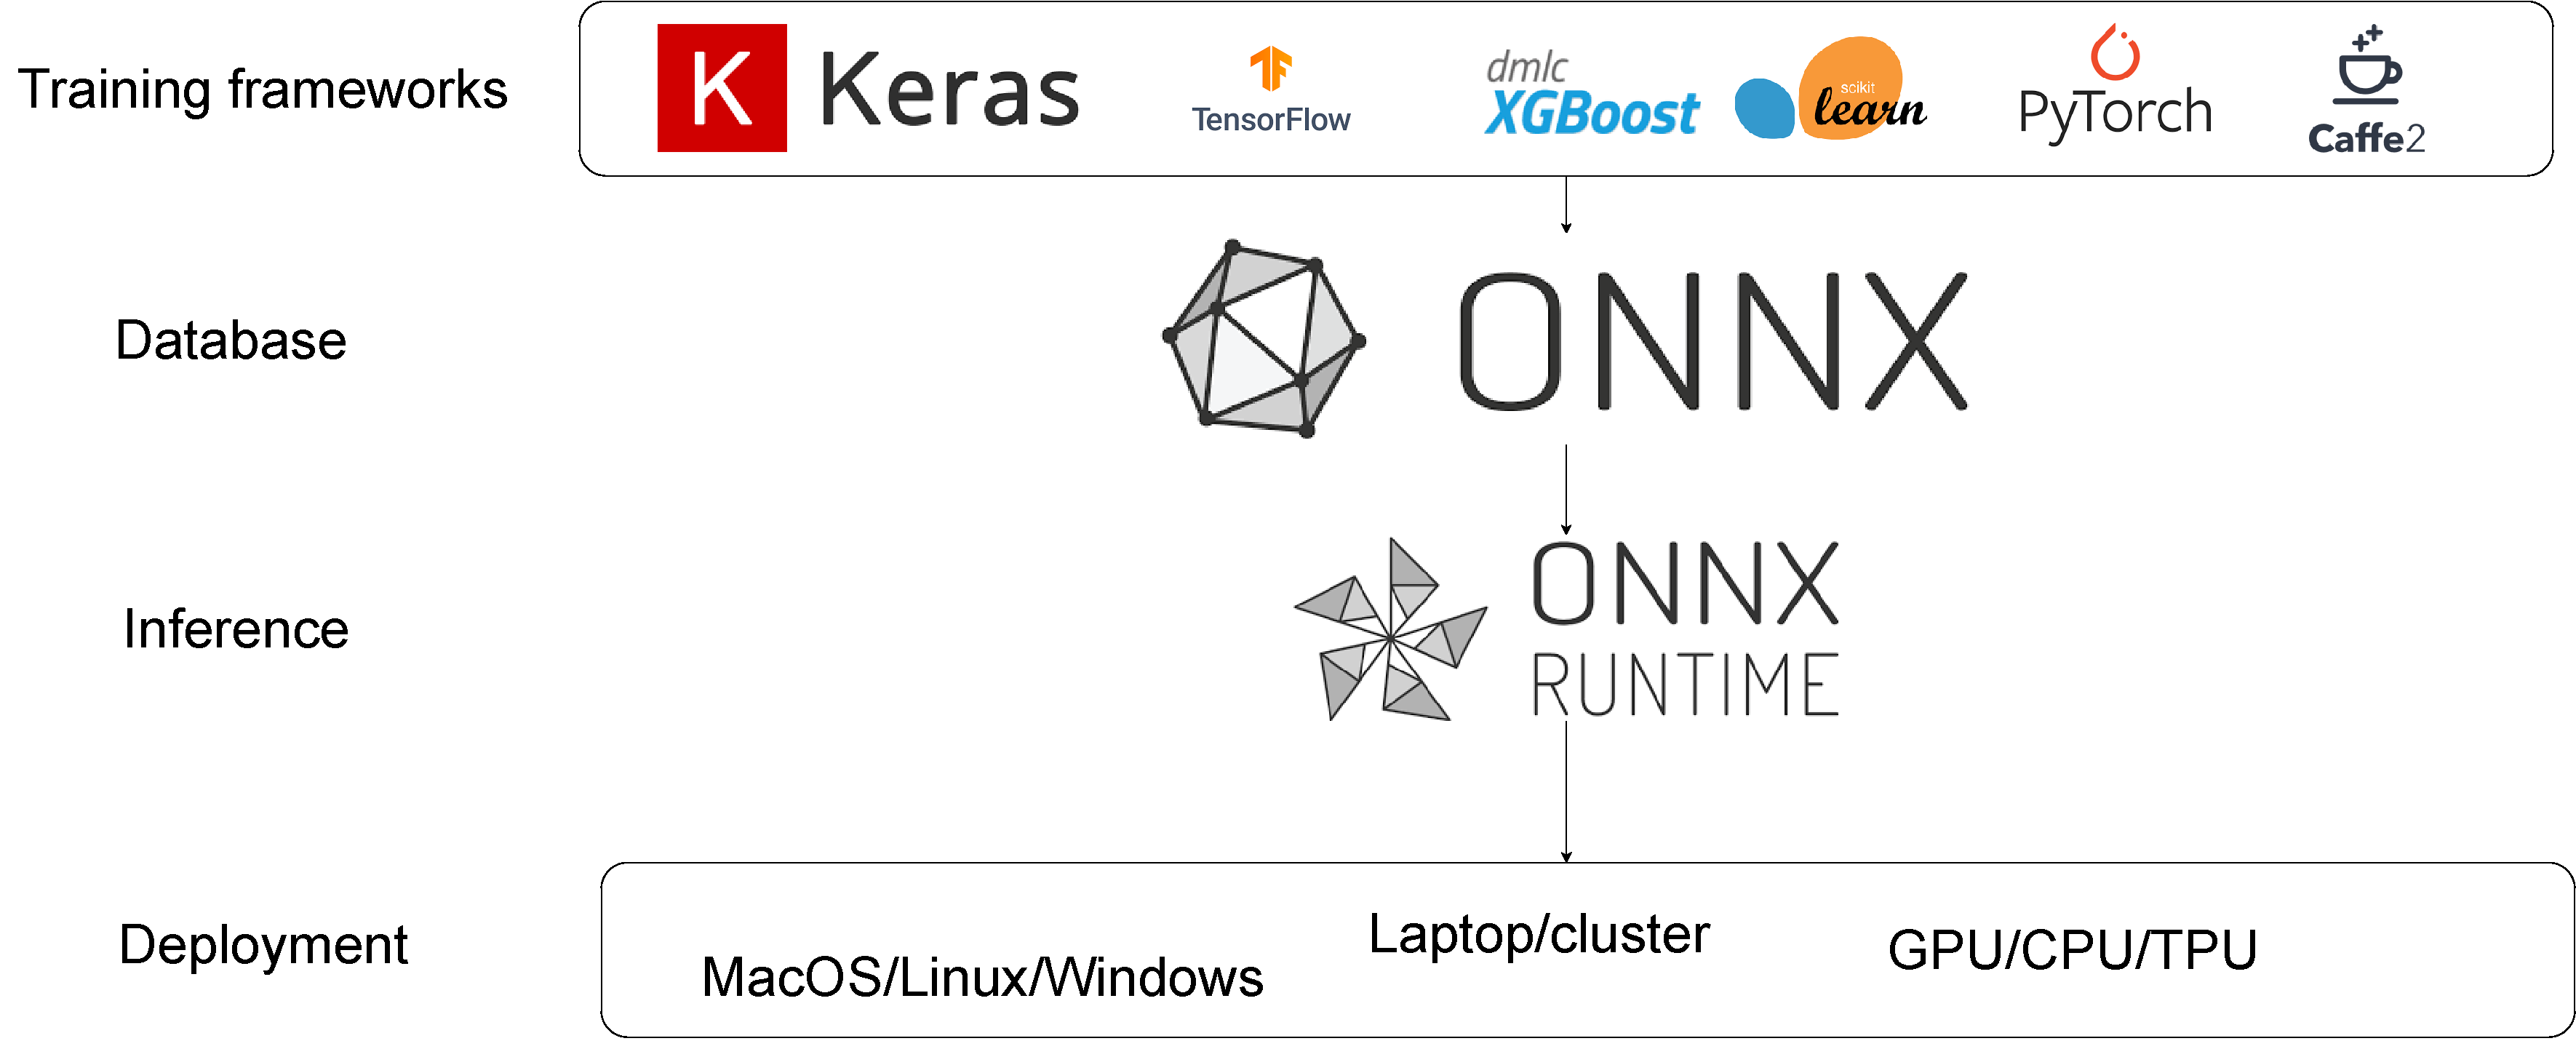
\includegraphics[width=.7\textwidth]{onix_workflow.pdf}\\\vspace*{.5cm}
    No accuracy loss due to conversion before interference!
    }
  \end{figure}
\end{frame}


\begin{frame}[t]{What is ONNX?}
  \begin{columns}
    \begin{column}{0.5\textwidth}
      \begin{itemize}
        \item Open Neural Network Exchange (ONNX)
        \item Support DNN and traditional ML models
        \item Cross-platform
        \item See \href{https://onnx.ai/supported-tools.html}{\color{blue} onnx.ai} for full list of supported frameworks
        \item Open source
      \end{itemize}
      \vspace*{1cm}
      ONNX and ONNX runtime:
      \begin{itemize}
        \item ONNX provides common representation for computational graph models
        \item ONNX runtime:
        \begin{itemize}
          \item Graph optimization
          \item Inference session
          % \item Execution - Sequential / Parallel
        \end{itemize}
      \end{itemize}
    \end{column}
    \begin{column}{0.5\textwidth}
      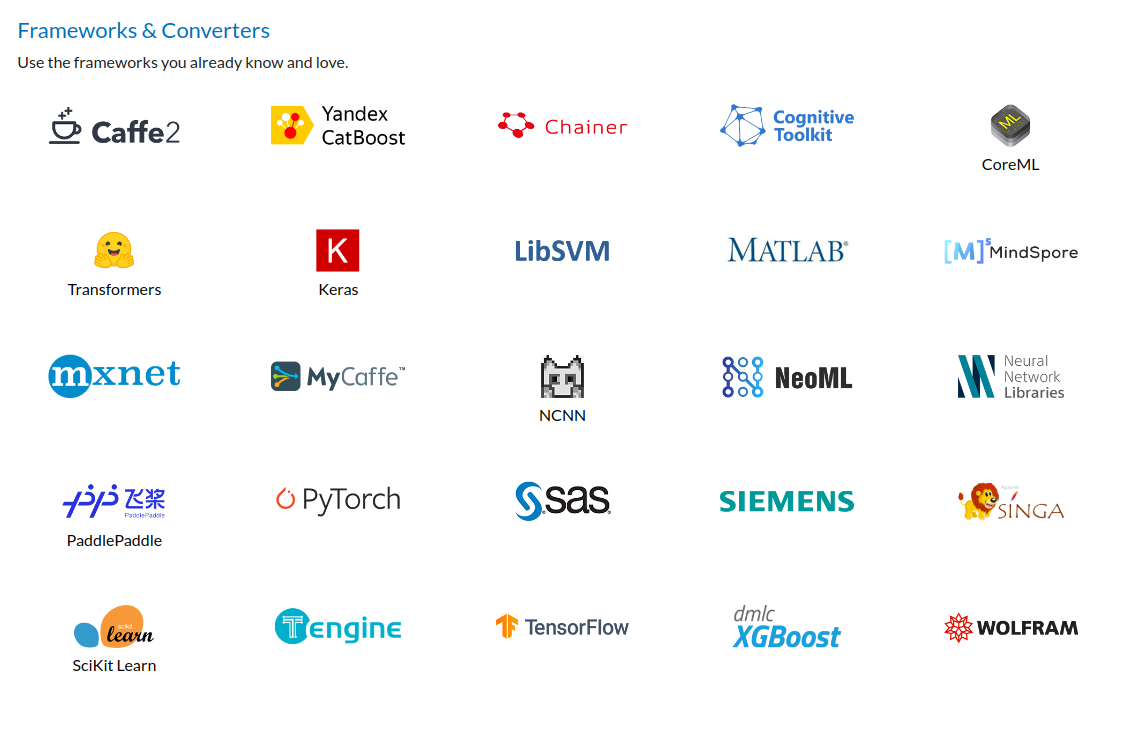
\includegraphics[width=.9\textwidth]{frameworks_converters.png}
    \end{column}
  \end{columns}
\end{frame}


% ONNX in practice =============================================================
\section{ONNX in practice}
\begin{frame}[t,fragile]{How to get ONNX model}
  Many tutorials with examples on the \href{https://github.com/onnx/tutorials\#converting-to-onnx-format}{\color{blue}onnx github page}\\
  \vspace*{1em}
  \textbf{Pytorch} (supports exporting to ONNX format):
  \begin{lstlisting}[language=Python]
    import torch.onnx
    import torchvision
    
    # Standard ImageNet input - 3 channels, 224x224,
    # values don't matter as we care about network structure.
    # But they can also be real inputs.
    dummy_input = torch.randn(1, 3, 224, 224)
    # Obtain your model, it can be also constructed in your script explicitly
    model = torchvision.models.alexnet(pretrained=True)
    # Invoke export
    torch.onnx.export(model, dummy_input, "alexnet.onnx")    
  \end{lstlisting}
\end{frame}


\begin{frame}[t,fragile]{How to get ONNX model}
  Many tutorials with examples on the \href{https://github.com/onnx/tutorials\#converting-to-onnx-format}{\color{blue}onnx github page}\\
  \vspace*{1em}
  \textbf{scikit-learn} (Not just neural networks):
  \begin{lstlisting}[language=Python]
    # Train a model.
    from sklearn.datasets import load_iris
    from sklearn.model_selection import train_test_split
    from sklearn.ensemble import RandomForestClassifier
    iris = load_iris()
    X, y = iris.data, iris.target
    X_train, X_test, y_train, y_test = train_test_split(X, y)
    clr = RandomForestClassifier()
    clr.fit(X_train, y_train)
    
    # Convert into ONNX format
    from skl2onnx import convert_sklearn
    from skl2onnx.common.data_types import FloatTensorType
    initial_type = [('float_input', FloatTensorType([None, 4]))]
    onx = convert_sklearn(clr, initial_types=initial_type)
    with open("rf_iris.onnx", "wb") as f:
        f.write(onx.SerializeToString())
  \end{lstlisting}
\end{frame}


\begin{frame}[t,fragile]{How to get ONNX model}
  Many tutorials with examples on the \href{https://github.com/onnx/tutorials\#converting-to-onnx-format}{\color{blue}onnx github page}\\
  \vspace*{1em}
  \textbf{TensorFlow:}
  \begin{lstlisting}[language=bash]
    python -m tf2onnx.convert --saved-model model --output onnx.model
  \end{lstlisting}
\end{frame}


\begin{frame}[t]{Standardized Model}
  \begin{columns}[t]
    \column{0.48\textwidth}
      \begin{itemize}
        \item Common operators and common file format
        \item Well documented
        \item \href{https://netron.app/}{\color{blue}netron.app} for model visualization
      \end{itemize}
    \column{0.48\textwidth}
      \begin{figure}
        \vspace*{-1.5cm}
        \centering
        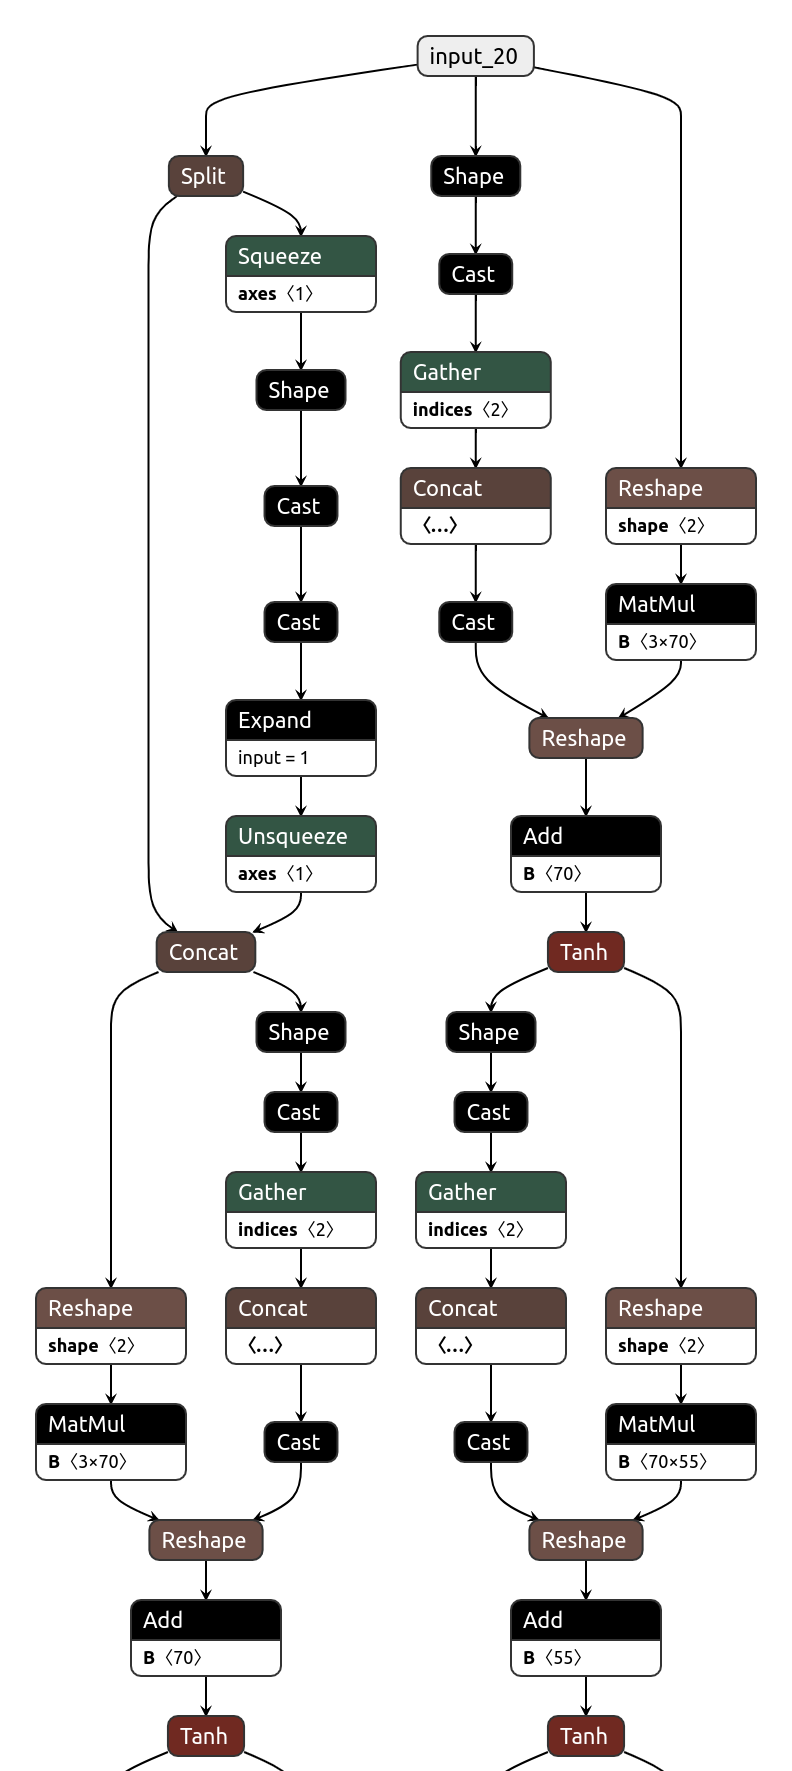
\includegraphics[height=0.95\textheight]{netron.png}
      \end{figure}
  \end{columns}
\end{frame}


\begin{frame}[t]{Deploy: ONNX runtime}{\color{blue} \href{https://onnxruntime.ai/}{onnxruntime.ai}}
  \begin{itemize}
    \item High performance interference engine for ONNX models
    \item Supports full ONNX-ML stack
    \item Extensive support for many hardware accelerators
    \item ONNX runtme optimizes for the target hardware \\
          (e.g. optimizing for TensorRt to run on an NVIDIA GPU)
  \end{itemize}
  \begin{figure}
    \centering
    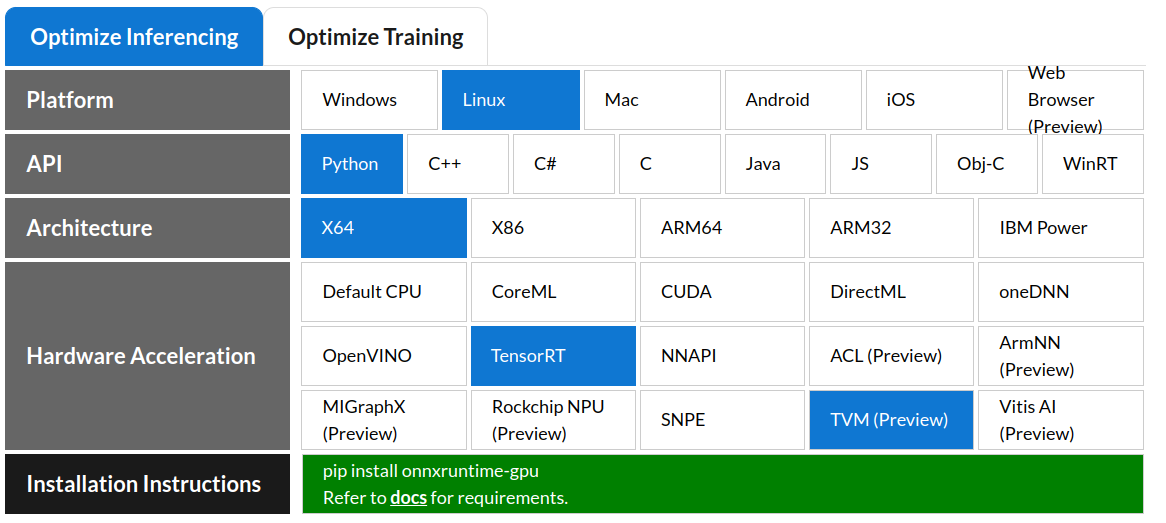
\includegraphics[width=.6\textwidth]{ONNX-runtime-get-started-chart.png}
  \end{figure}
\end{frame}


\begin{frame}[t,fragile]{Easily load ONNX model with ONNX runtime for inference:}
  \vspace*{1em}
  \textbf{scikit-learn:}
  \begin{lstlisting}[language=Python]
    # Compute the prediction with ONNX Runtime
    import onnxruntime as rt
    import numpy
    sess = rt.InferenceSession("rf_iris.onnx")
    input_name = sess.get_inputs()[0].name
    label_name = sess.get_outputs()[0].name
    pred_onx = sess.run([label_name], {input_name: X_test.astype(numpy.float32)})[0]
  \end{lstlisting}
\end{frame}


% CONCLUSIONS ==================================================================
\section{Conclusions}
\begin{frame}[t]{Not an original idea}
  \begin{columns}
    \column{.48\textwidth}
      ATLAS already made \href{https://github.com/lwtnn/lwtnn}{\color{blue}\underline{Lightweight Trained Neural Network (LWTNN)}},
      \begin{itemize}
        \item convert NN to standard JSON format
        \item reconstruct NN for C++ development
      \end{itemize}
      however..
      \begin{itemize}
        \item supports a much more limited selection of models (subset of scikit and Keras)
        \item development is less active (arguably a positive\ldots)
        \item limited to C++
      \end{itemize}
    \column{.48\textwidth}
      \begin{figure}
        \centering
        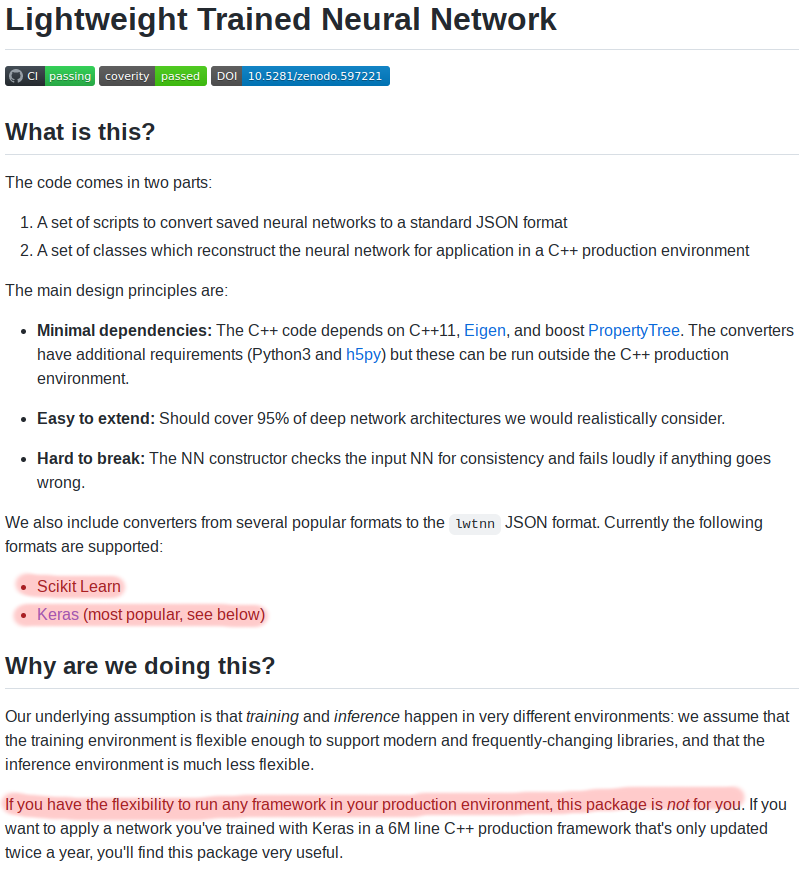
\includegraphics[width=.8\textwidth]{screenshot_lwtnn.png}
      \end{figure}
  \end{columns}
\end{frame}

\begin{frame}[t]{Conclusions}
  \begin{itemize}
    \item Physicists work in small teams borrowing from each other
    \item Every tool is slightly different
    \item but many shared features (models, data, visualization)
    \item yet much time is spend on plugging everything together
    \item while sometimes even losing prediction accuracy during model conversion
  \end{itemize}
  \vspace*{.5cm}
  Stop re-re-reinventing the wheel: use standardized open-source tools from ML communities such as ONNX where possible\\\vspace*{1cm}
  \only<2>{
    \begin{center}
      \bfseries Thank you!
    \end{center}
  }
\end{frame}


\begin{frame}{Determination of the photon PDF}
  \begin{columns}[T]
    \begin{column}{0.59\textwidth}
      Initially the photon PDF has been determined in different ways:
      \begin{itemize}
        \item physical model: sensitive to underlying model
        \item fitting: data does not provide strong constraints
      \end{itemize}

      \vspace*{0.5em}
      However with the LUXqed approach it can be computed perturbatively \\
      based on the observation that the heavy-lepton production cross-section can be written in two ways:
      \begin{itemize}
        \item in terms of structure functions $F_2$, $F_L$
        \item in terms of PDFs (including the photon)
      \end{itemize}

      \vspace*{0.5em}
      luxQED result {\color{gray}\small[Manohar, Nason, Salam, Zanderighi: 1607.04266, 1708.01256]}:
      \vspace*{-0.8em}
      \begin{equation*}
        \begin{split}
          & x \gamma(x, \mu^2)
          =
          \frac{2}{\alpha (\mu^2)} \int\limits_x^1 \frac{dz}{z}
          \Biggl\{ \int_{m_p^2x^2 \over 1-z}^{\mu^2 \over 1-z} \frac{dQ^2}{Q^2}
          \alpha^2(Q^2) \Biggl[ -z^2 F_L(x/z, Q^2) \\
          & + \left( z P_{\gamma q}(z) + \frac{2 x^2 m_p^2}{Q^2} \right)
          F_2(x/z, Q^2)\Biggr] - \alpha^2(\mu^2) z^2 F_2(x/z, \mu^2)\Biggr\}
        \end{split}
      \end{equation*}
    \end{column}

    \begin{column}{0.39\textwidth}
      \vspace*{-2.5em}
      \begin{figure}
        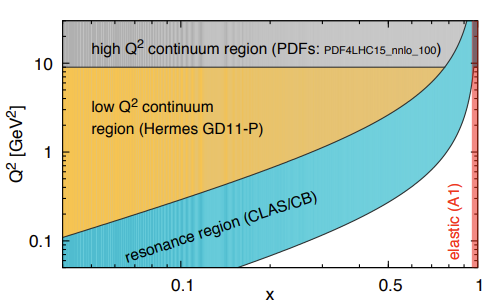
\includegraphics[width=0.89\textwidth]{figures/dataluxqed.png}
        \caption*{Input to construct $F_2$ and $F_L$}
        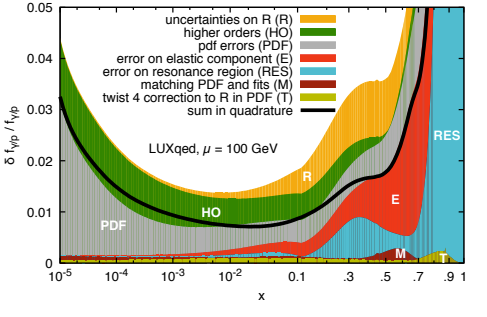
\includegraphics[width=0.89\textwidth]{figures/luxQED_uncs.png}
        \caption*{Sources of uncertainty}
      \end{figure}
    \end{column}
  \end{columns}
\end{frame}


\begin{frame}{LUXqed PDF determinations}
  LUXqed has been used in all of the most recent QED PDFs:
  \begin{itemize}
      \item LUXqed\_plus\_PDF4LHC15 {\color{gray}\small [1607.04266]}
      \item LUXqed17\_plus\_PDF4LHC15 {\color{gray}\small [1708.01256]}
      \item MMHT2015qed {\color{gray}\small [1907.02750]}
      \item NNPDF3.1luxQED {\color{gray}\small [1712.07053]}
      \item CT18lux and CT18qed {\color{gray}\small [2106.10299]}
      \item MSHT20QED {\color{gray}\small [2111.05357]}
      \item MSHT20qed\_an3lo {\color{gray}\small [2312.07665]}
      \item NNPDF4.0QED {\color{gray}\small [2401.08749 ]}
  \end{itemize}
\end{frame}

% \begin{frame}{Results: photon PDF and luminosity}
%   \begin{center}
%     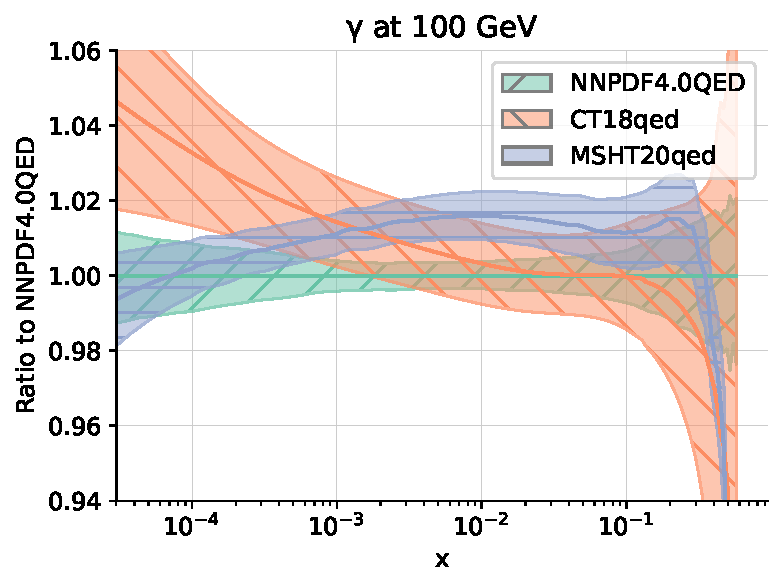
\includegraphics[width=0.3\textwidth]{figures/photon_comparison.pdf}
%     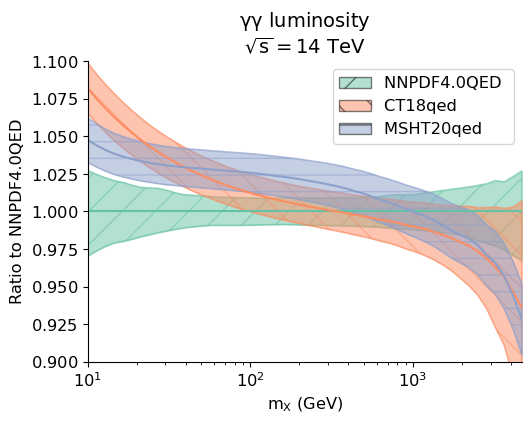
\includegraphics[width=0.3\textwidth]{figures/pp_lumi_comparison.png}
%     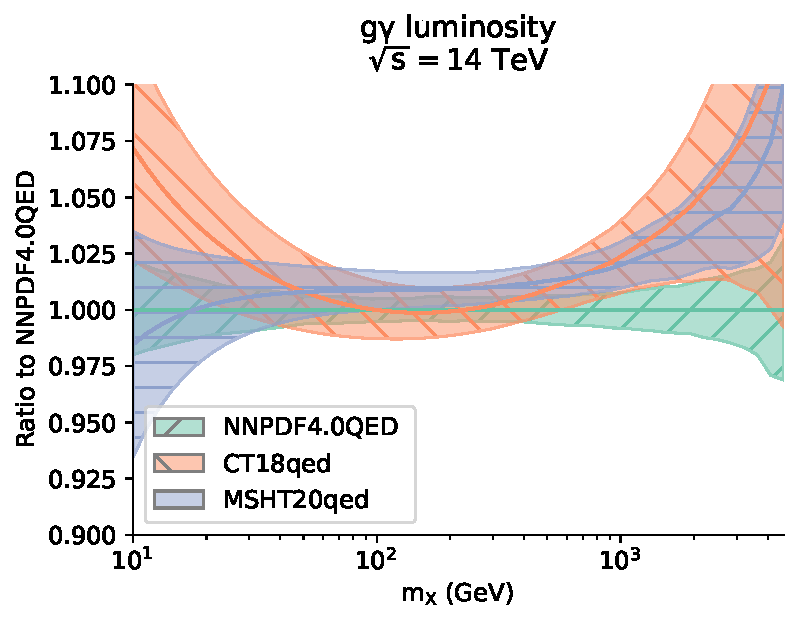
\includegraphics[width=0.3\textwidth]{figures/gp_lumi_comparison.pdf}
%   \end{center}
%   \begin{itemize}
%     \item Because all groups use the luxQED formalism, the photon PDFs agree at percent level
%     \item Luminosity generally in agreement, but differ at very small and very large invariant mass
%   \end{itemize}
% \end{frame}


% ============================================================================


\begin{frame}{Incomplete higher order uncertainties covmat}
  \begin{itemize}
    \item We construct an IHOU matrix following a similar approach by varying the subleading functions
    \item IHOU are independent of MHOU so the uncertainties are added in quadrature
    $$C = C_\mathrm{exp}+C_\mathrm{MHOU}+C_\mathrm{IHOU}$$
  \end{itemize}

  \begin{columns}
    \begin{column}{0.49\textwidth}
      \begin{figure}[!t]
        \centering
        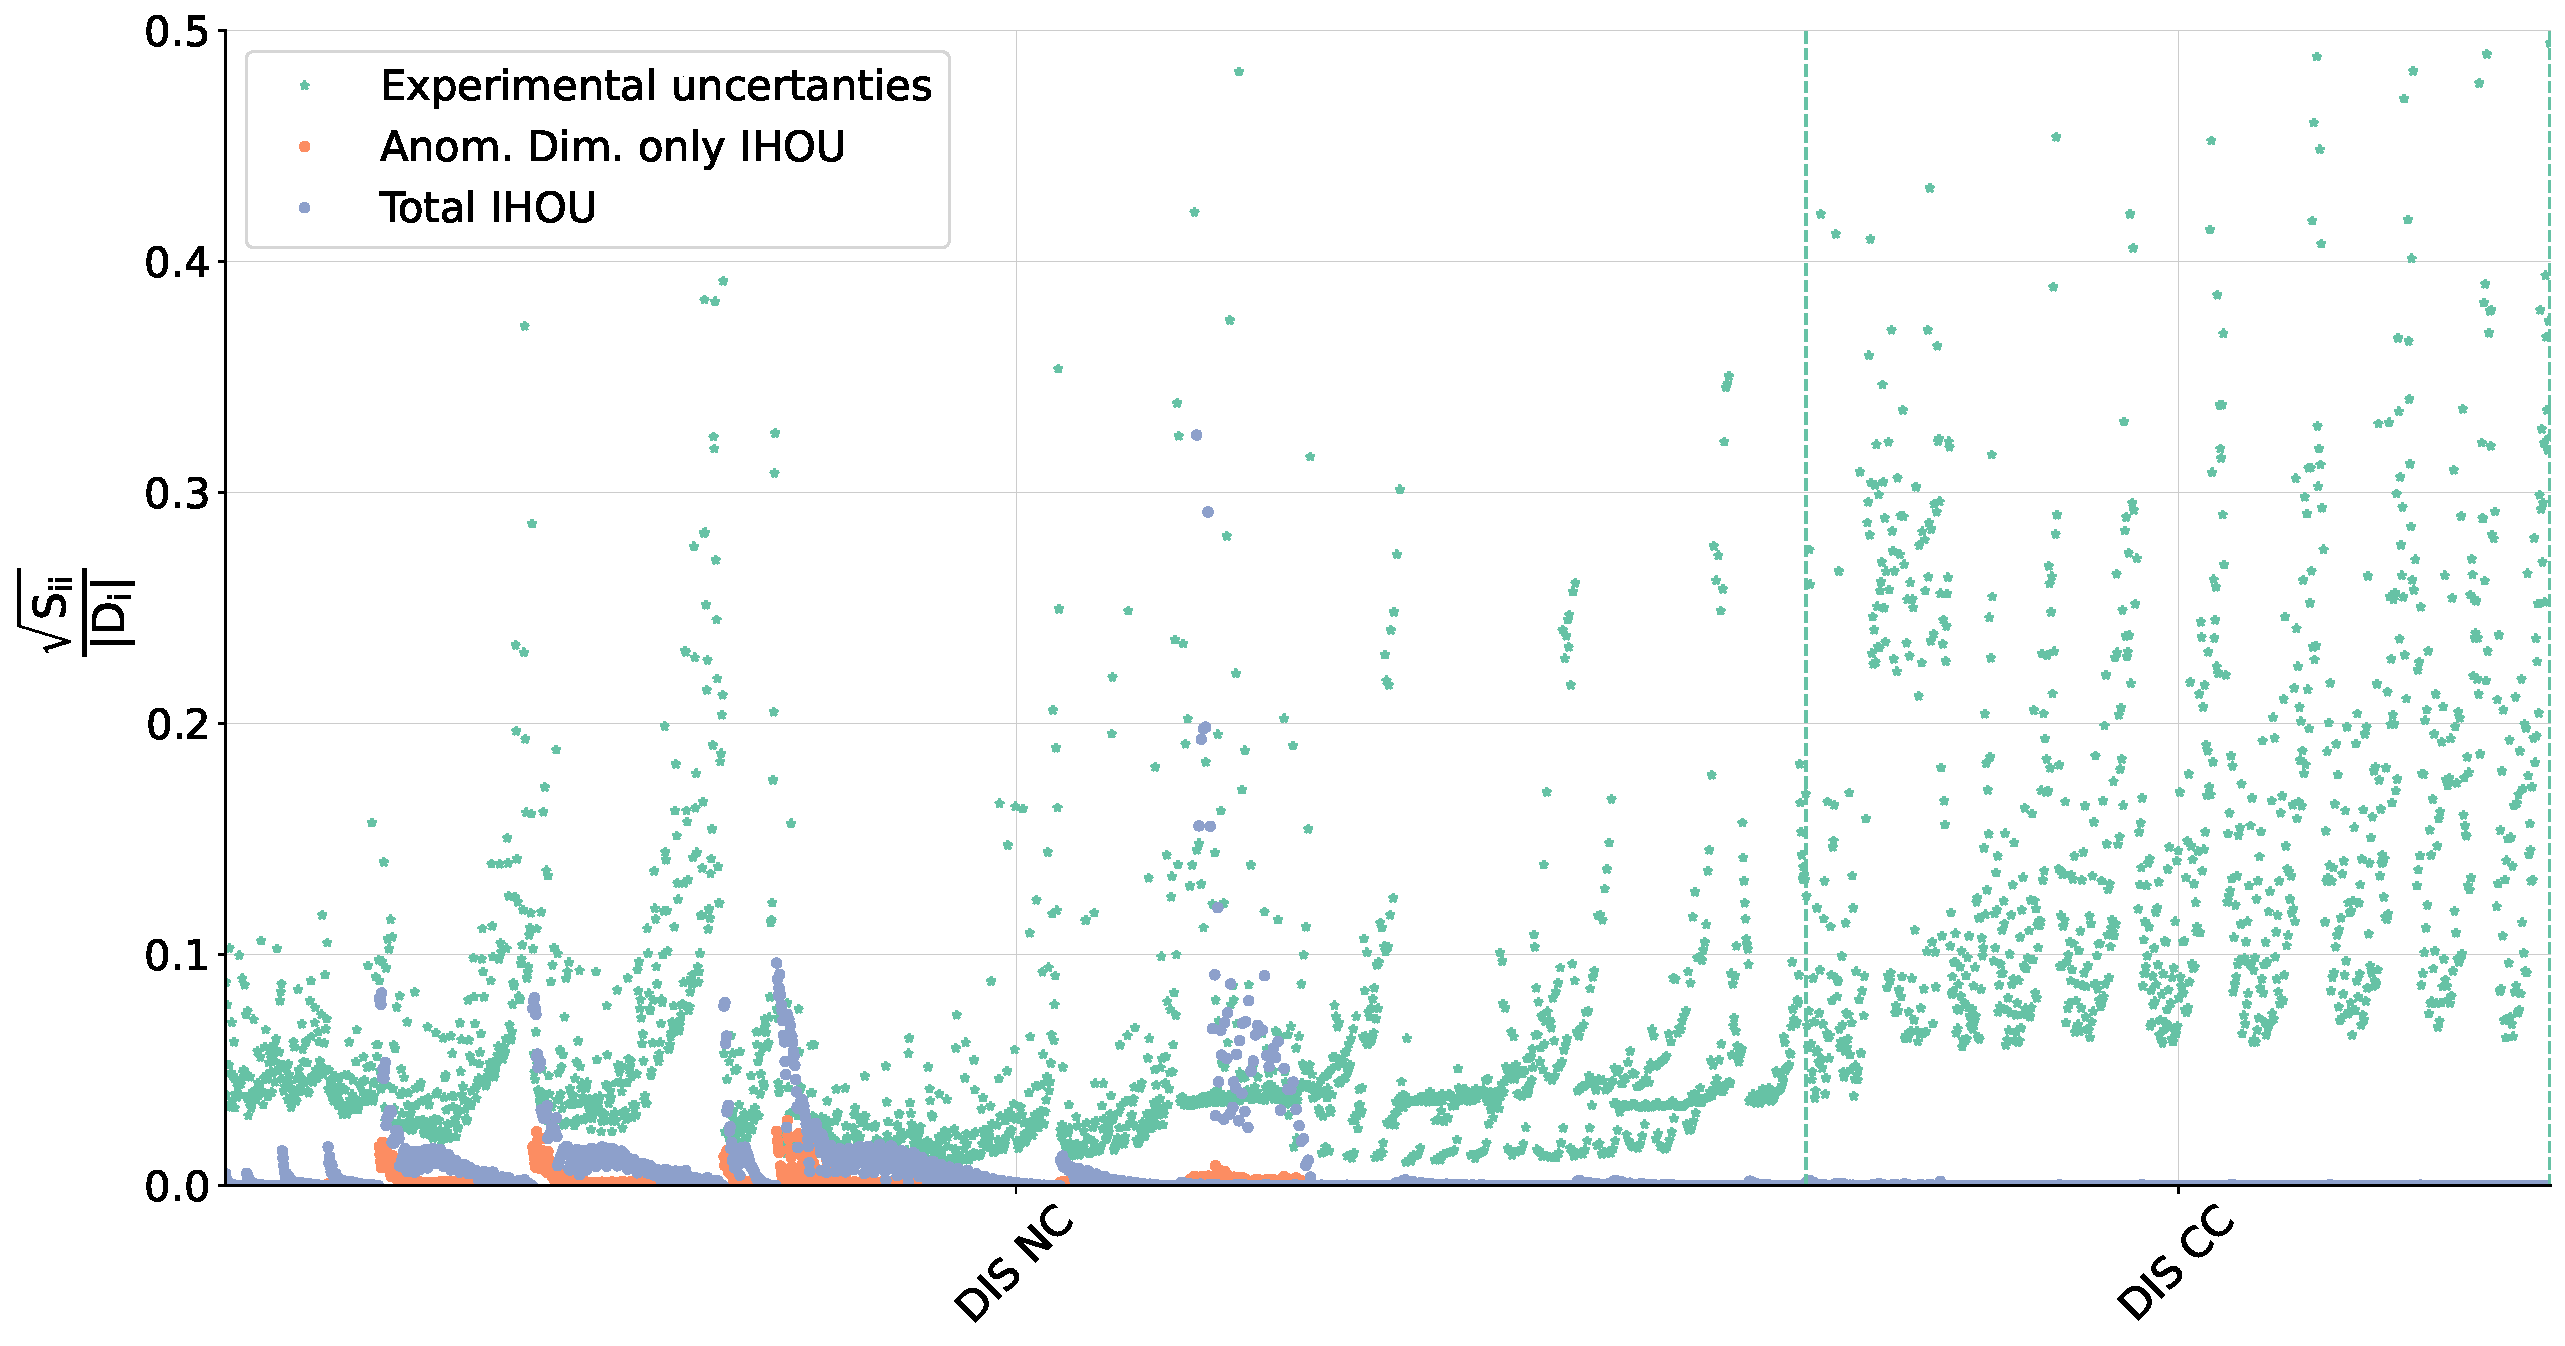
\includegraphics[width=.9\textwidth]{figures/diag_cov_dis_ihou.pdf}
        \caption*{IHOU have a large effect on small-$x$, low-$Q$ DIS data
        }
      \end{figure}
    \end{column}
    \begin{column}{0.49\textwidth}
      \begin{figure}[!t]
        \centering
        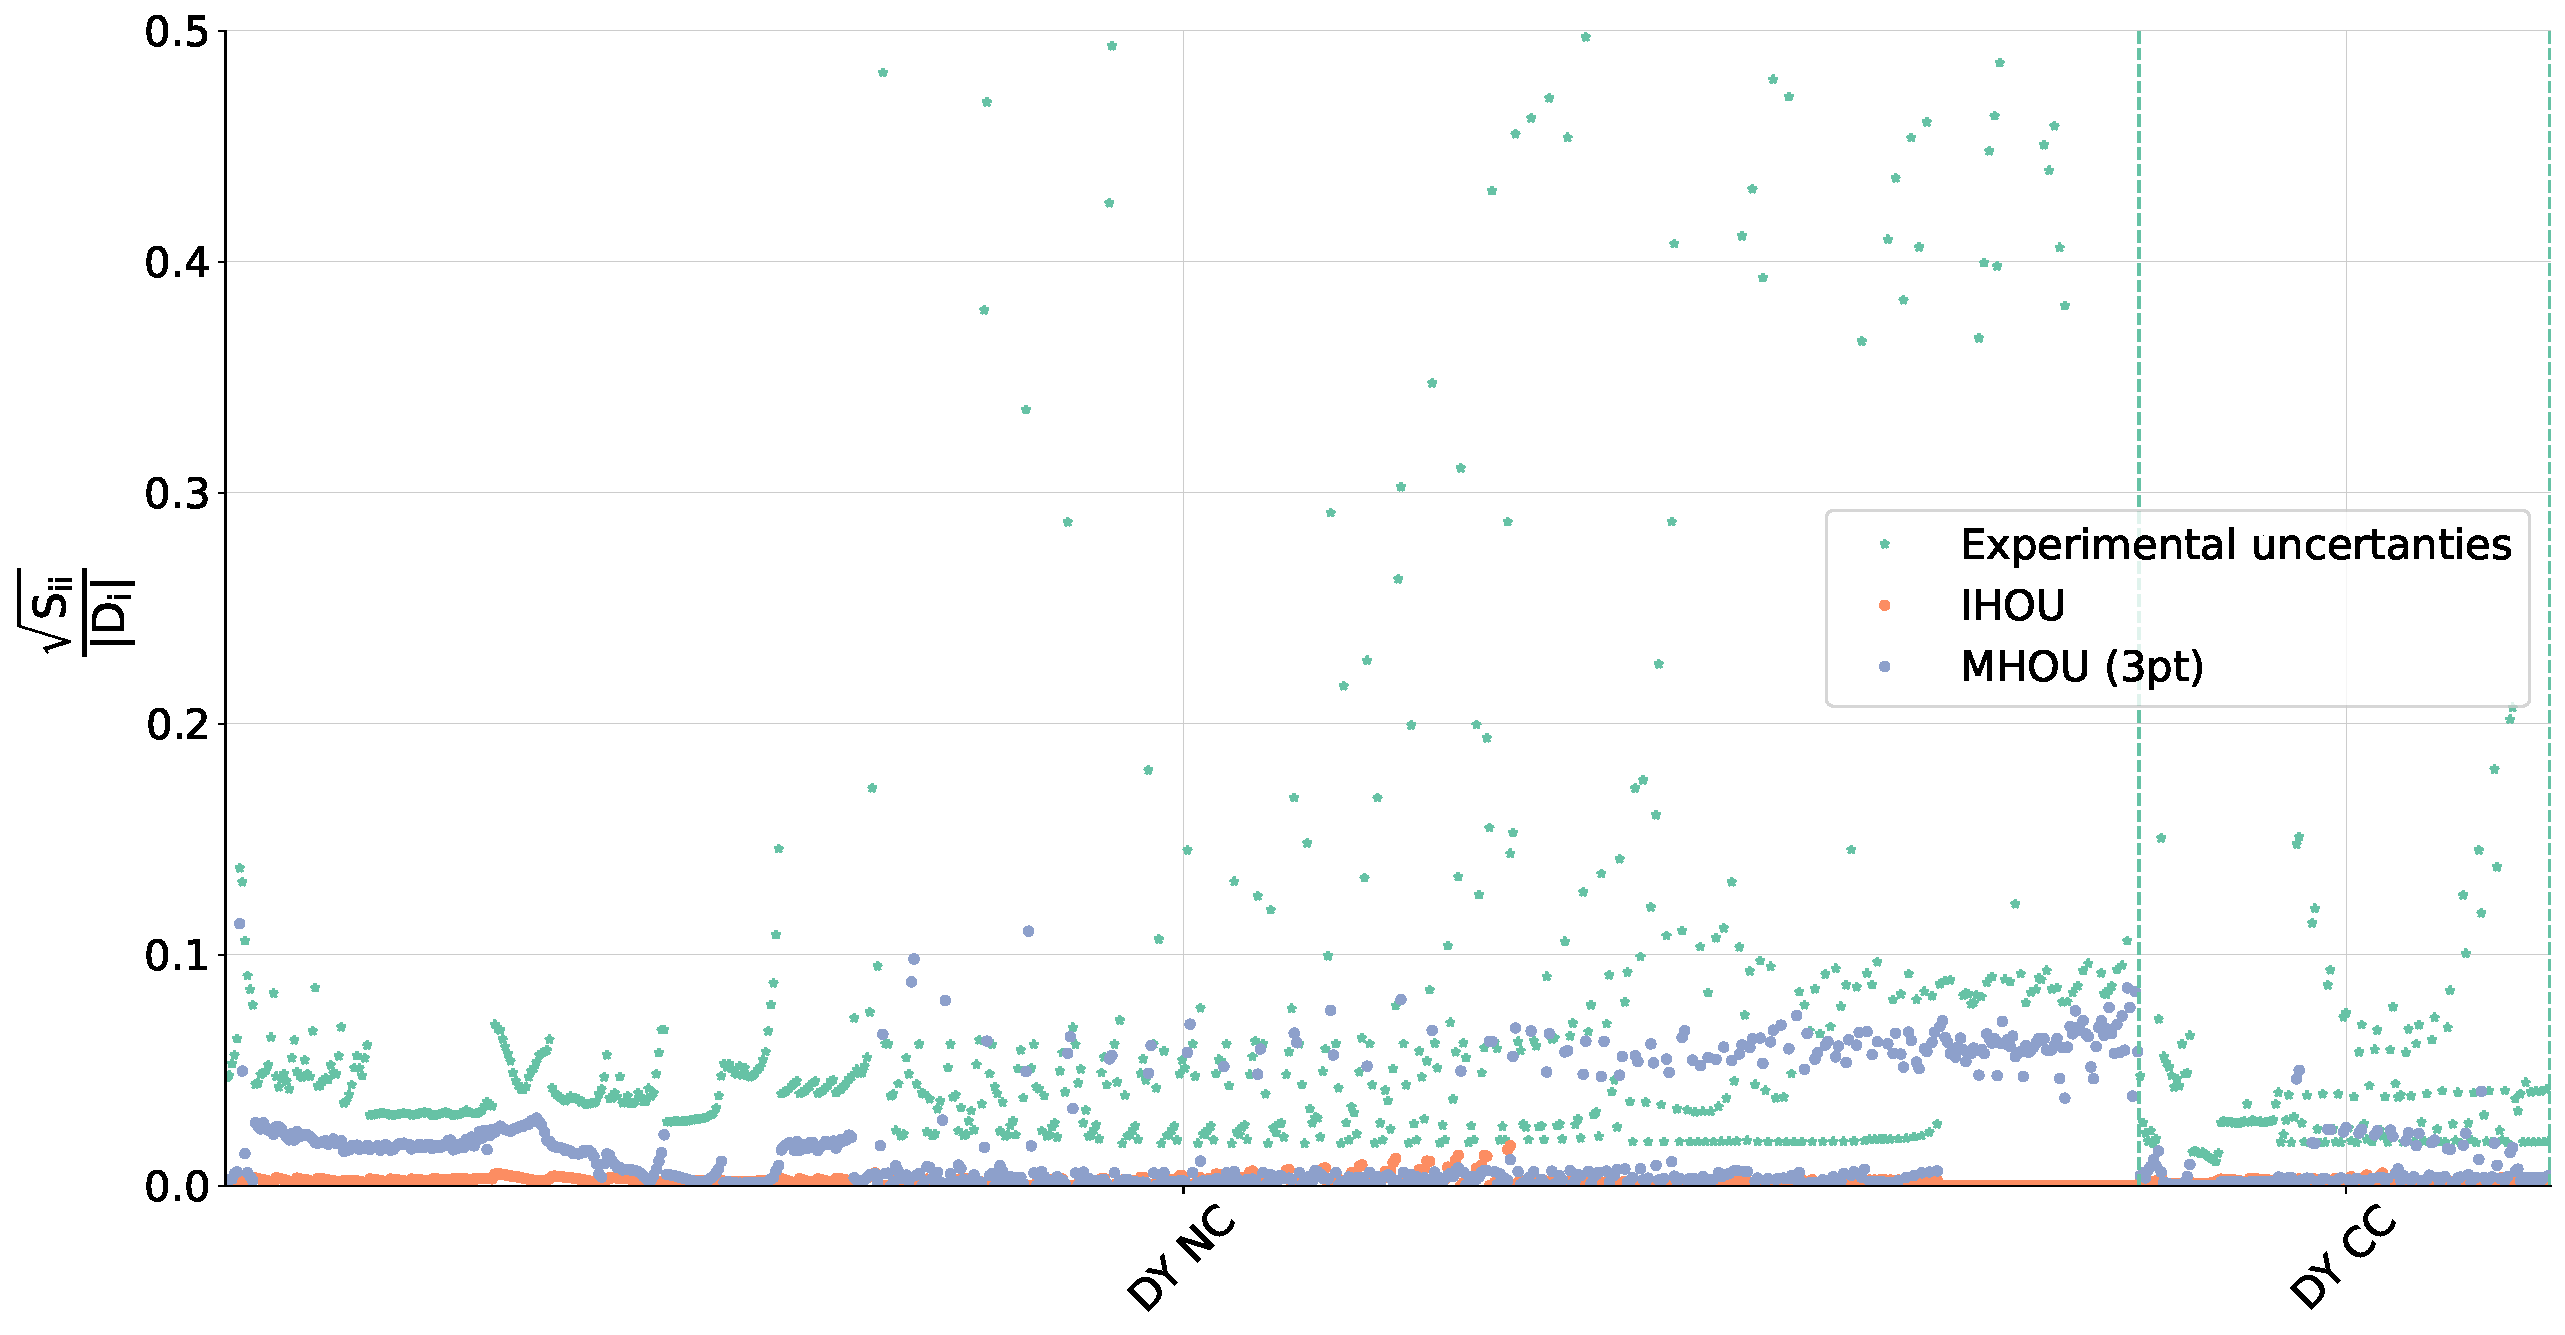
\includegraphics[width=.9\textwidth]{figures/diag_cov_dy_ihou_3pt_mhou.pdf}
        \caption*{NNLO MHOU included where N3LO not available \\
          MHOU can similar magnitude as the experimental uncertainty
        }
      \end{figure}
    \end{column}
  \end{columns}


\end{frame}

% \begin{frame}{Magnitude of theory uncertainties}
% % show that for certain processes th unc is of same size as exp unc.
% \end{frame}

% ============================================================================

\begin{frame}{Impact of MHOUs at N3LO}
  \begin{figure}[!t]
    \centering
    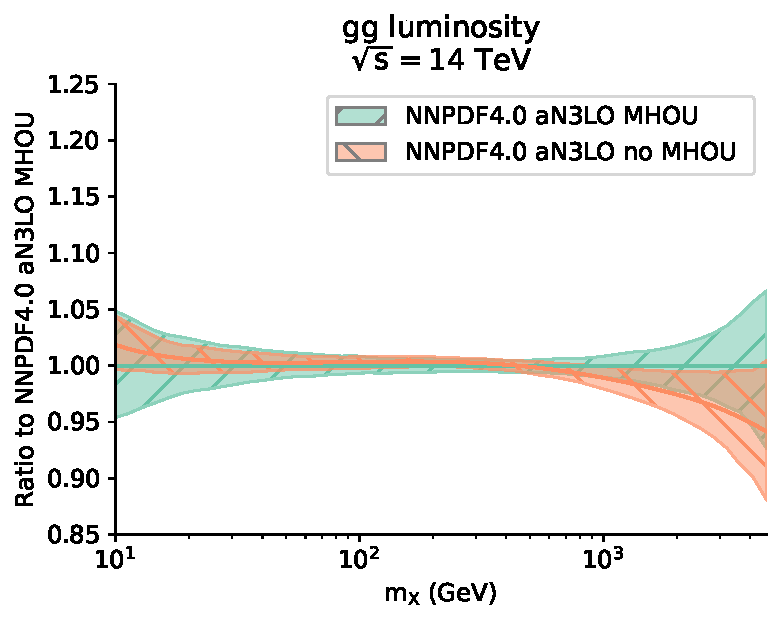
\includegraphics[width=0.45\textwidth]{figures/gg_plot_lumi1d.pdf}
    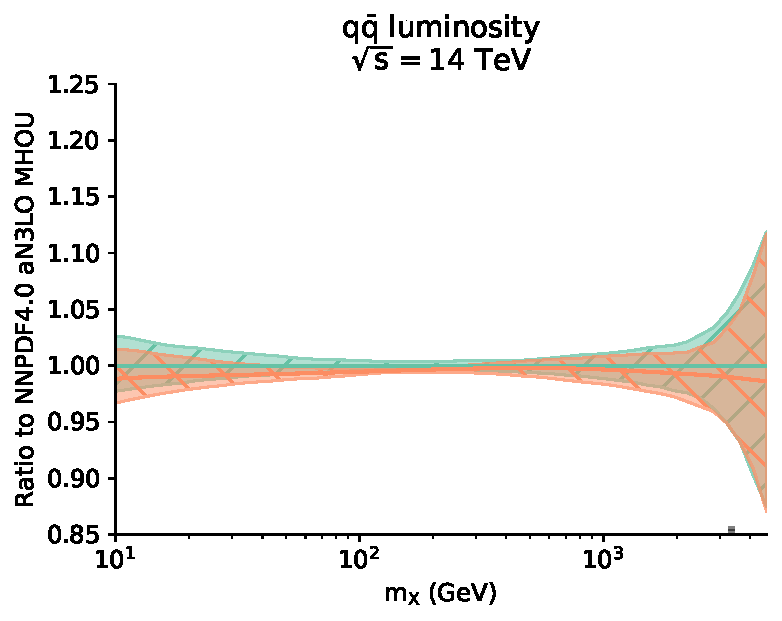
\includegraphics[width=0.45\textwidth]{figures/qqbar_plot_lumi1d.pdf}
  \end{figure}
  \begin{itemize}
    \item Non-negligible impact of MHOUs even at N3LO
    \item[$\Rightarrow$] reason to include exact N3LO calculations for hadronic processes
  \end{itemize}
\end{frame}


% \begin{frame}{Comparison to MSHT20}
%   \begin{figure}[!t]
%     \centering
%     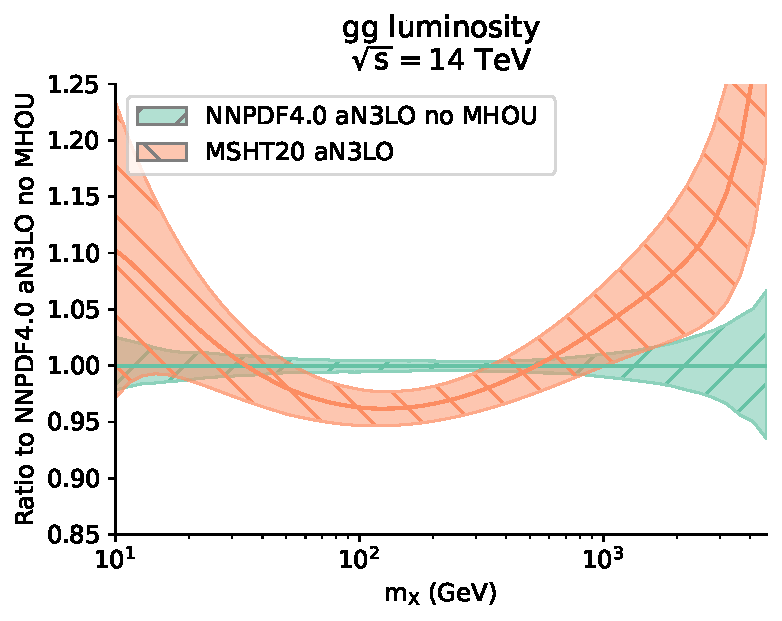
\includegraphics[width=0.45\textwidth]{figures/gg_plot_lumi1d_msht20.pdf}
%     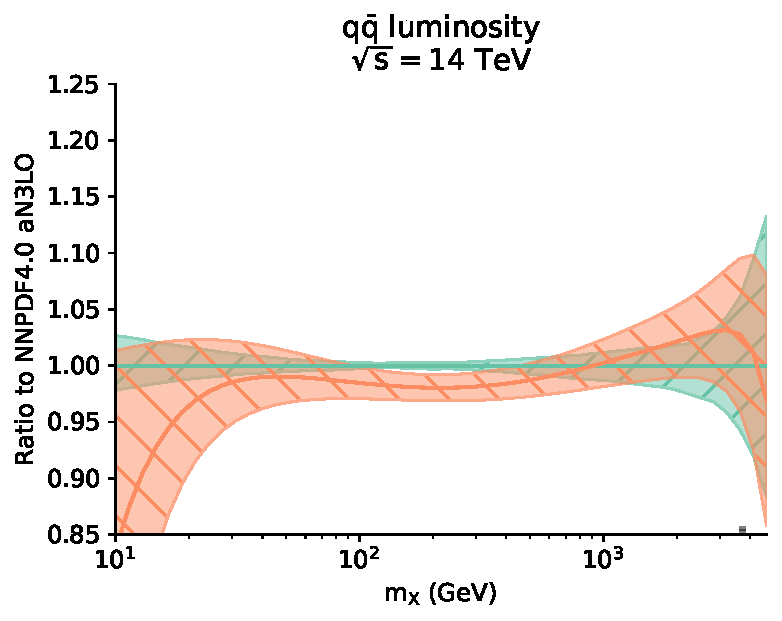
\includegraphics[width=0.45\textwidth]{figures/qqbar_plot_lumi1d_msht20.pdf}
%   \end{figure}
%   \begin{itemize}
%     \item Good agreement with MSHT20 for the quark luminosities
%     \item Also for gluon luminosities, except around the Higgs mass and high-mass
%     \item Similar data but different methodology (including splitting function parametrization)
%   \end{itemize}
% \end{frame}



\end{document}
